\documentclass[14pt]{extbook}
\usepackage{multicol, enumerate, enumitem, hyperref, color, soul, setspace, parskip, fancyhdr} %General Packages
\usepackage{amssymb, amsthm, amsmath, latexsym, units, mathtools} %Math Packages
\everymath{\displaystyle} %All math in Display Style
% Packages with additional options
\usepackage[headsep=0.5cm,headheight=12pt, left=1 in,right= 1 in,top= 1 in,bottom= 1 in]{geometry}
\usepackage[usenames,dvipsnames]{xcolor}
\usepackage{dashrule}  % Package to use the command below to create lines between items
\newcommand{\litem}[1]{\item#1\hspace*{-1cm}\rule{\textwidth}{0.4pt}}
\pagestyle{fancy}
\lhead{Makeup Progress Quiz 2}
\chead{}
\rhead{Version A}
\lfoot{5763-3522}
\cfoot{}
\rfoot{Spring 2021}
\begin{document}

\begin{enumerate}
\litem{
Solve the equation below. Then, choose the interval that contains the solution.\[ -17(8x + 19) = -3(7x + 4) \]\begin{enumerate}[label=\Alph*.]
\item \( x \in [-2.94, -2.77] \)
\item \( x \in [-2.43, -1.77] \)
\item \( x \in [-2.82, -2.7] \)
\item \( x \in [2.65, 3.32] \)
\item \( \text{There are no real solutions.} \)

\end{enumerate} }
\litem{
First, find the equation of the line containing the two points below. Then, write the equation as $ y=mx+b $ and choose the intervals that contain $m$ and $b$.\[ (-11, 8) \text{ and } (-3, -10) \]\begin{enumerate}[label=\Alph*.]
\item \( m \in [-3.25, -1.25] \hspace*{3mm} b \in [-8, -5] \)
\item \( m \in [-3.25, -1.25] \hspace*{3mm} b \in [19, 22] \)
\item \( m \in [-3.25, -1.25] \hspace*{3mm} b \in [10.75, 17.75] \)
\item \( m \in [-3.25, -1.25] \hspace*{3mm} b \in [-19.75, -10.75] \)
\item \( m \in [2.25, 3.25] \hspace*{3mm} b \in [-5.25, -0.25] \)

\end{enumerate} }
\litem{
Find the equation of the line described below. Write the linear equation as $ y=mx+b $ and choose the intervals that contain $m$ and $b$.\[ \text{Parallel to } 4 x - 9 y = 4 \text{ and passing through the point } (4, -9). \]\begin{enumerate}[label=\Alph*.]
\item \( m \in [1.68, 3.26] \hspace*{3mm} b \in [-11.78, -8.78] \)
\item \( m \in [-0.34, 1.17] \hspace*{3mm} b \in [8.78, 15.78] \)
\item \( m \in [-1.16, 0.19] \hspace*{3mm} b \in [-8.22, -6.22] \)
\item \( m \in [-0.34, 1.17] \hspace*{3mm} b \in [-14, -11] \)
\item \( m \in [-0.34, 1.17] \hspace*{3mm} b \in [-11.78, -8.78] \)

\end{enumerate} }
\litem{
Write the equation of the line in the graph below in Standard form $Ax+By=C$. Then, choose the intervals that contain $A, B, \text{ and } C$.
\begin{center}
    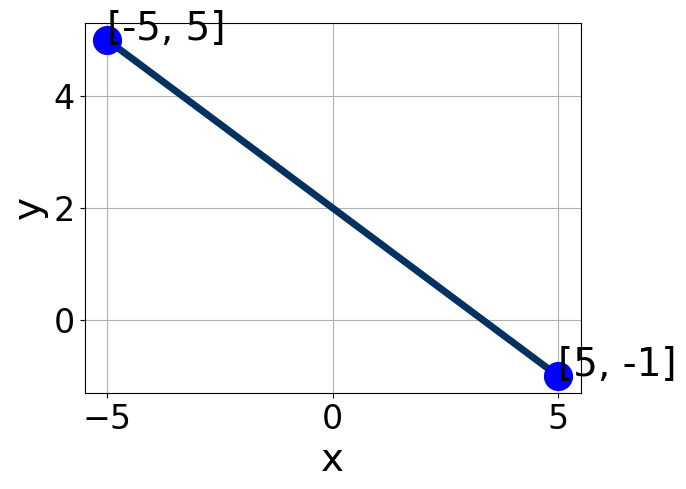
\includegraphics[width=0.5\textwidth]{../Figures/linearGraphToStandardCopyA.png}
\end{center}
\begin{enumerate}[label=\Alph*.]
\item \( A \in [-5.6, -1.2], \hspace{3mm} B \in [-5.77, -4.68], \text{ and } \hspace{3mm} C \in [-10, -3] \)
\item \( A \in [2.7, 6.5], \hspace{3mm} B \in [4.47, 5.8], \text{ and } \hspace{3mm} C \in [7, 13] \)
\item \( A \in [-0.6, 1.2], \hspace{3mm} B \in [0.82, 2.26], \text{ and } \hspace{3mm} C \in [0, 6] \)
\item \( A \in [2.7, 6.5], \hspace{3mm} B \in [-5.77, -4.68], \text{ and } \hspace{3mm} C \in [-10, -3] \)
\item \( A \in [-0.6, 1.2], \hspace{3mm} B \in [-1.91, 0.15], \text{ and } \hspace{3mm} C \in [-9, 1] \)

\end{enumerate} }
\litem{
Write the equation of the line in the graph below in Standard form $Ax+By=C$. Then, choose the intervals that contain $A, B, \text{ and } C$.
\begin{center}
    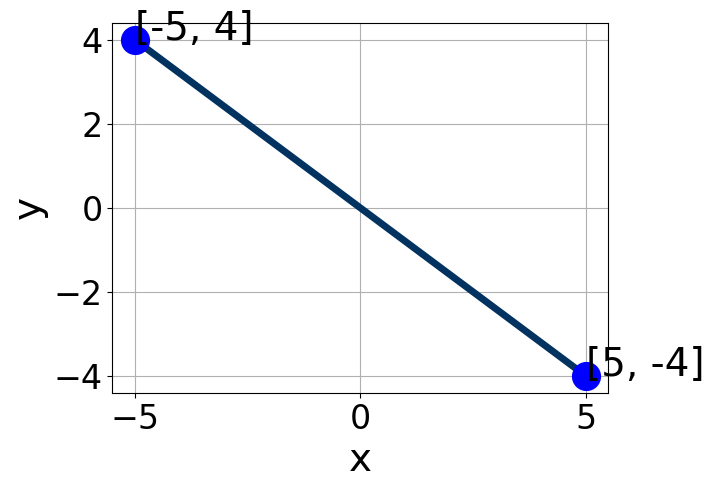
\includegraphics[width=0.5\textwidth]{../Figures/linearGraphToStandardA.png}
\end{center}
\begin{enumerate}[label=\Alph*.]
\item \( A \in [1, 7], \hspace{3mm} B \in [4, 5.99], \text{ and } \hspace{3mm} C \in [-2, 3] \)
\item \( A \in [-2.2, 2.8], \hspace{3mm} B \in [0.71, 2.09], \text{ and } \hspace{3mm} C \in [-2, 3] \)
\item \( A \in [1, 7], \hspace{3mm} B \in [-5.96, -3.24], \text{ and } \hspace{3mm} C \in [-2, 3] \)
\item \( A \in [-2.2, 2.8], \hspace{3mm} B \in [-1.33, 0.02], \text{ and } \hspace{3mm} C \in [-2, 3] \)
\item \( A \in [-7, -2], \hspace{3mm} B \in [-5.96, -3.24], \text{ and } \hspace{3mm} C \in [-2, 3] \)

\end{enumerate} }
\litem{
Solve the linear equation below. Then, choose the interval that contains the solution.\[ \frac{3x + 6}{7} - \frac{6x -7}{4} = \frac{-6x -4}{5} \]\begin{enumerate}[label=\Alph*.]
\item \( x \in [-1.2, 0.5] \)
\item \( x \in [-132.4, -131.5] \)
\item \( x \in [-27.3, -25.7] \)
\item \( x \in [-0.7, 0.9] \)
\item \( \text{There are no real solutions.} \)

\end{enumerate} }
\litem{
Find the equation of the line described below. Write the linear equation as $ y=mx+b $ and choose the intervals that contain $m$ and $b$.\[ \text{Parallel to } 8 x + 3 y = 3 \text{ and passing through the point } (-2, -7). \]\begin{enumerate}[label=\Alph*.]
\item \( m \in [-3.1, -1.5] \hspace*{3mm} b \in [12.33, 14.33] \)
\item \( m \in [-3.1, -1.5] \hspace*{3mm} b \in [-14.33, -9.33] \)
\item \( m \in [0.5, 5] \hspace*{3mm} b \in [-1.67, 0.33] \)
\item \( m \in [-3.1, -1.5] \hspace*{3mm} b \in [-9, -4] \)
\item \( m \in [-1.1, 0.5] \hspace*{3mm} b \in [-14.33, -9.33] \)

\end{enumerate} }
\litem{
Solve the equation below. Then, choose the interval that contains the solution.\[ -9(-16x + 7) = -12(-6x -10) \]\begin{enumerate}[label=\Alph*.]
\item \( x \in [0.72, 0.89] \)
\item \( x \in [-0.88, -0.68] \)
\item \( x \in [-0.7, -0.25] \)
\item \( x \in [2.29, 3.12] \)
\item \( \text{There are no real solutions.} \)

\end{enumerate} }
\litem{
First, find the equation of the line containing the two points below. Then, write the equation as $ y=mx+b $ and choose the intervals that contain $m$ and $b$.\[ (8, 6) \text{ and } (6, 5) \]\begin{enumerate}[label=\Alph*.]
\item \( m \in [-0.49, 1.04] \hspace*{3mm} b \in [-2.5, -1.4] \)
\item \( m \in [-0.49, 1.04] \hspace*{3mm} b \in [-2.5, -1.4] \)
\item \( m \in [-0.49, 1.04] \hspace*{3mm} b \in [1, 4.5] \)
\item \( m \in [-0.49, 1.04] \hspace*{3mm} b \in [-1.6, -0.3] \)
\item \( m \in [-1.51, -0.45] \hspace*{3mm} b \in [6.5, 8.8] \)

\end{enumerate} }
\litem{
Solve the linear equation below. Then, choose the interval that contains the solution.\[ \frac{-5x -8}{6} - \frac{-4x -4}{3} = \frac{3x + 7}{2} \]\begin{enumerate}[label=\Alph*.]
\item \( x \in [-4.5, -2.5] \)
\item \( x \in [-9.17, -4.17] \)
\item \( x \in [-1.88, 1.12] \)
\item \( x \in [-14, -8] \)
\item \( \text{There are no real solutions.} \)

\end{enumerate} }
\end{enumerate}

\end{document}